\documentclass[tikz,border=5pt]{standalone}
\usepackage{tikz, amsmath}
\usetikzlibrary{arrows.meta, calc}

\begin{document}


%% ================================================================
%% Figure 2 – Redistribution: two-step cell → segment → vertex
%% ================================================================
%%
%% V1=(1.8,2.8) inside cell (0,1)   V2=(4.3,2.2) inside cell (2,1)
%% Segment midpoints:
%%   sigma1: mid((0,1.5),(1.8,2.8))  = (0.90, 2.15)
%%   sigma2: mid((1.8,2.8),(4.3,2.2)) = (3.05, 2.50)
%%   sigma3: mid((4.3,2.2),(6,3.5))  = (5.15, 2.85)
%%
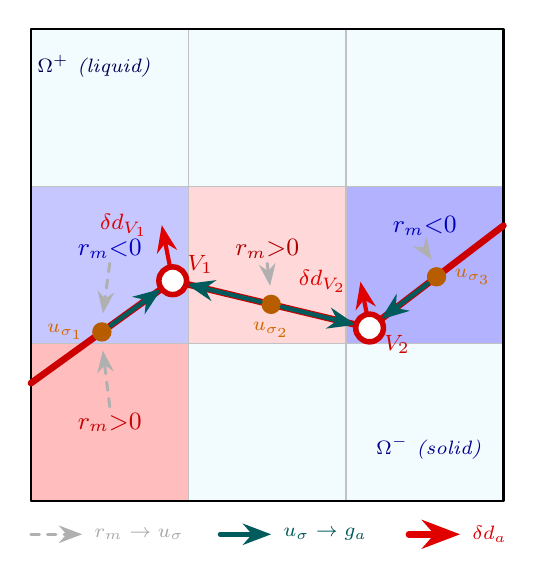
\begin{tikzpicture}[>=Stealth, font=\small, line cap=round, line join=round]

  %% ---- background + cell residual colors ----
  \fill[cyan!5]   (0,0) rectangle (6,6);
  \fill[red!26]   (0,0) rectangle (2,2);
  \fill[blue!22]  (0,2) rectangle (2,4);
  \fill[red!15]   (2,2) rectangle (4,4);
  \fill[blue!30]  (4,2) rectangle (6,4);

  %% ---- grid ----
  \draw[gray!48, thin] (0,0) grid[step=2] (6,6);
  \draw[black, thick] (0,0) rectangle (6,6);

  %% ---- front ----
  \draw[red!80!black, line width=2.4pt]
    (0,1.5) -- (1.8,2.8) -- (4.3,2.2) -- (6,3.5);

  %% ---- residual labels ----
  \node[red!78!black,  font=\small\bfseries] at (1.00,1.00) {$r_m{>}0$};
  \node[blue!78!black, font=\small\bfseries] at (1.00,3.20) {$r_m{<}0$};
  \node[red!68!black,  font=\small\bfseries] at (3.00,3.20) {$r_m{>}0$};
  \node[blue!72!black, font=\small\bfseries] at (5.00,3.50) {$r_m{<}0$};

  %% ---- segment midpoints ----
  \fill[orange!72!black] (0.90,2.15) circle (3.5pt);
  \node[left=3pt, font=\scriptsize, orange!82!black] at (0.90,2.15) {$u_{\sigma_1}$};
  \fill[orange!72!black] (3.05,2.50) circle (3.5pt);
  \node[below=3pt, font=\scriptsize, orange!82!black] at (3.05,2.50) {$u_{\sigma_2}$};
  \fill[orange!72!black] (5.15,2.85) circle (3.5pt);
  \node[right=3pt, font=\scriptsize, orange!82!black] at (5.15,2.85) {$u_{\sigma_3}$};

  %% ---- Step 1: cell -> segment midpoint (gray dashed) ----
  \draw[->, gray!62, dashed, line width=1.1pt, shorten >=3pt]
    (1.00,1.20) -- (0.90,2.02);
  \draw[->, gray!62, dashed, line width=1.1pt, shorten >=3pt]
    (1.00,3.02) -- (0.90,2.28);
  \draw[->, gray!62, dashed, line width=1.1pt, shorten >=3pt]
    (3.00,3.02) -- (3.05,2.63);
  \draw[->, gray!62, dashed, line width=1.1pt, shorten >=3pt]
    (5.00,3.2) -- (5.15,2.98);

  %% ---- Step 2: segment midpoint -> vertex (teal) ----
  \draw[->, teal!72!black, line width=1.6pt, shorten <=4pt, shorten >=5pt]
    (0.90,2.15) -- (1.80,2.80);
  \draw[->, teal!72!black, line width=1.6pt, shorten <=4pt, shorten >=5pt]
    (3.05,2.50) -- (1.80,2.80);
  \draw[->, teal!72!black, line width=1.6pt, shorten <=4pt, shorten >=5pt]
    (3.05,2.50) -- (4.30,2.20);
  \draw[->, teal!72!black, line width=1.6pt, shorten <=4pt, shorten >=5pt]
    (5.15,2.85) -- (4.30,2.20);

  %% ---- vertex correction arrows (bold red) ----
  %% Normal at V1/V2 reused from figure 1: n ~ (-0.193, 0.981)
  \draw[->, red!88!black, line width=1.5pt]
    (1.8,2.8) -- ++({-0.193*0.72},{0.981*0.72})
    node[left=1pt, font=\footnotesize] {$\delta d_{V_1}$};
  \draw[->, red!88!black, line width=1.5pt]
    (4.3,2.2) -- ++({-0.193*0.60},{0.981*0.60})
    node[left=1pt, font=\footnotesize] {$\delta d_{V_2}$};

  %% ---- front vertex markers ----
  \foreach \x/\y in {1.8/2.8, 4.3/2.2}{
    \fill[white] (\x,\y) circle (5pt);
    \draw[red!82!black, line width=2pt] (\x,\y) circle (5pt);
  }
  \node[above right=-1pt, font=\footnotesize, red!82!black] at (1.9,2.8)  {$V_1$};
  \node[below right=-1pt, font=\footnotesize, red!82!black] at (4.4,2.2) {$V_2$};

  %% ---- phase labels ----
  \node[blue!55!black, font=\scriptsize\itshape] at (5.05,0.68) {$\Omega^-$ (solid)};
  \node[blue!32!black, font=\scriptsize\itshape] at (0.80,5.52) {$\Omega^+$ (liquid)};

  %% ---- compact legend ----
  \draw[->, gray!62, dashed, line width=1.2pt] (0.0,-0.42) -- (0.65,-0.42);
  \node[right, font=\scriptsize, gray!68] at (0.68,-0.42) {$r_m \to u_\sigma$};
  \draw[->, teal!72!black, line width=1.6pt]   (2.4,-0.42) -- (3.05,-0.42);
  \node[right, font=\scriptsize, teal!68!black] at (3.08,-0.42) {$u_\sigma \to g_a$};
  \draw[->, red!88!black, line width=2.4pt]    (4.8,-0.42) -- (5.45,-0.42);
  \node[right, font=\scriptsize, red!88!black]  at (5.48,-0.42) {$\delta d_a$};


\end{tikzpicture}

\end{document}
